
%---------------------------------------------------------------------

\chapter{Einleitung}

%---------------------------------------------------------------------


Mit dem Forschungsprojekt \gls{IKC} als Grundlage beschäftigt sich die vorliegende Arbeit vertieft mit der Analyse von Datenquellen und der Extraktion von relevanten Informationen. Aktuell werden Datenquellen verknüpft, jedoch wird deren Inhalt noch nirgends genutzt. 

Mit der Analyse dieser Inhalte werden zusätzliche Informationen Teil des Wissensnetzwerks. Dadurch wird aus einer reinen Verknüpfung von Datenquellen eine tatsächliche Integration der Informationen.

% % Dieser sorgt einerseits für eine Aufwertung des Informationsgehalts und andererseits soll er den Benutzer in der Verwendung des Prototyps unterstützen.

%Die Auswertung der Datenquellen ermöglicht dem Benutzer eine plattformübergreifende Volltextsuche und präsentiert ihm, anhand des jeweiligen Inhalts, eine Auswahl der relevanten Begriffe. Dadurch wird aus einer reinen Verknüpfung von Datenquellen eine tatsächliche Integration der Informationen.

Zum besseren Verständnis werden potentiell unbekannte oder pro\-jekt-spezifische Begriffe kursiv und fett dargestellt. Zu jedem Begriff ist eine kurze Beschreibung im Glossar (\hyperref[glossar]{Kapitel Glossar}) am Ende der Dokumentation zu finden. Im Anhang sind neben der Aufgabenstellung (\autoref{aufgabenstellung}) auch die wichtigsten Sitzungsprotokolle (\autoref{protokolle}) und das Arbeitsjounrnal (\autoref{arbeitsjournal}) beigelegt. Der dokumentierte Sourcecode\footnote{\url{https://gitlab.enterpriselab.ch/ikc}} ist auf dem entsprechenden Repository der Hochschule Luzern verfügbar.

%---------------------------------------------------------------------

\section{Ausgangslage}

%---------------------------------------------------------------------


\autoref{fig:kontextdiagramm} zeigt den Kontext des zu entwicklenden Prototypen. Der Benutzer arbeitet wie anhin mit dem \gls{ikc-core}. Dieser wird aber vor allem im Hintergrund aber auch in der Benutzeroberfläche auf die neue Funktionalität hin angepasst und optimiert. Der Prototyp nimmt Anfragen für \gls{Keyphrase}[s] und für Suchresultate für den entsprechenden Begriff entgegen und liefert die angeforderten Resultate zurück.

\begin{figure}[H]
\centering
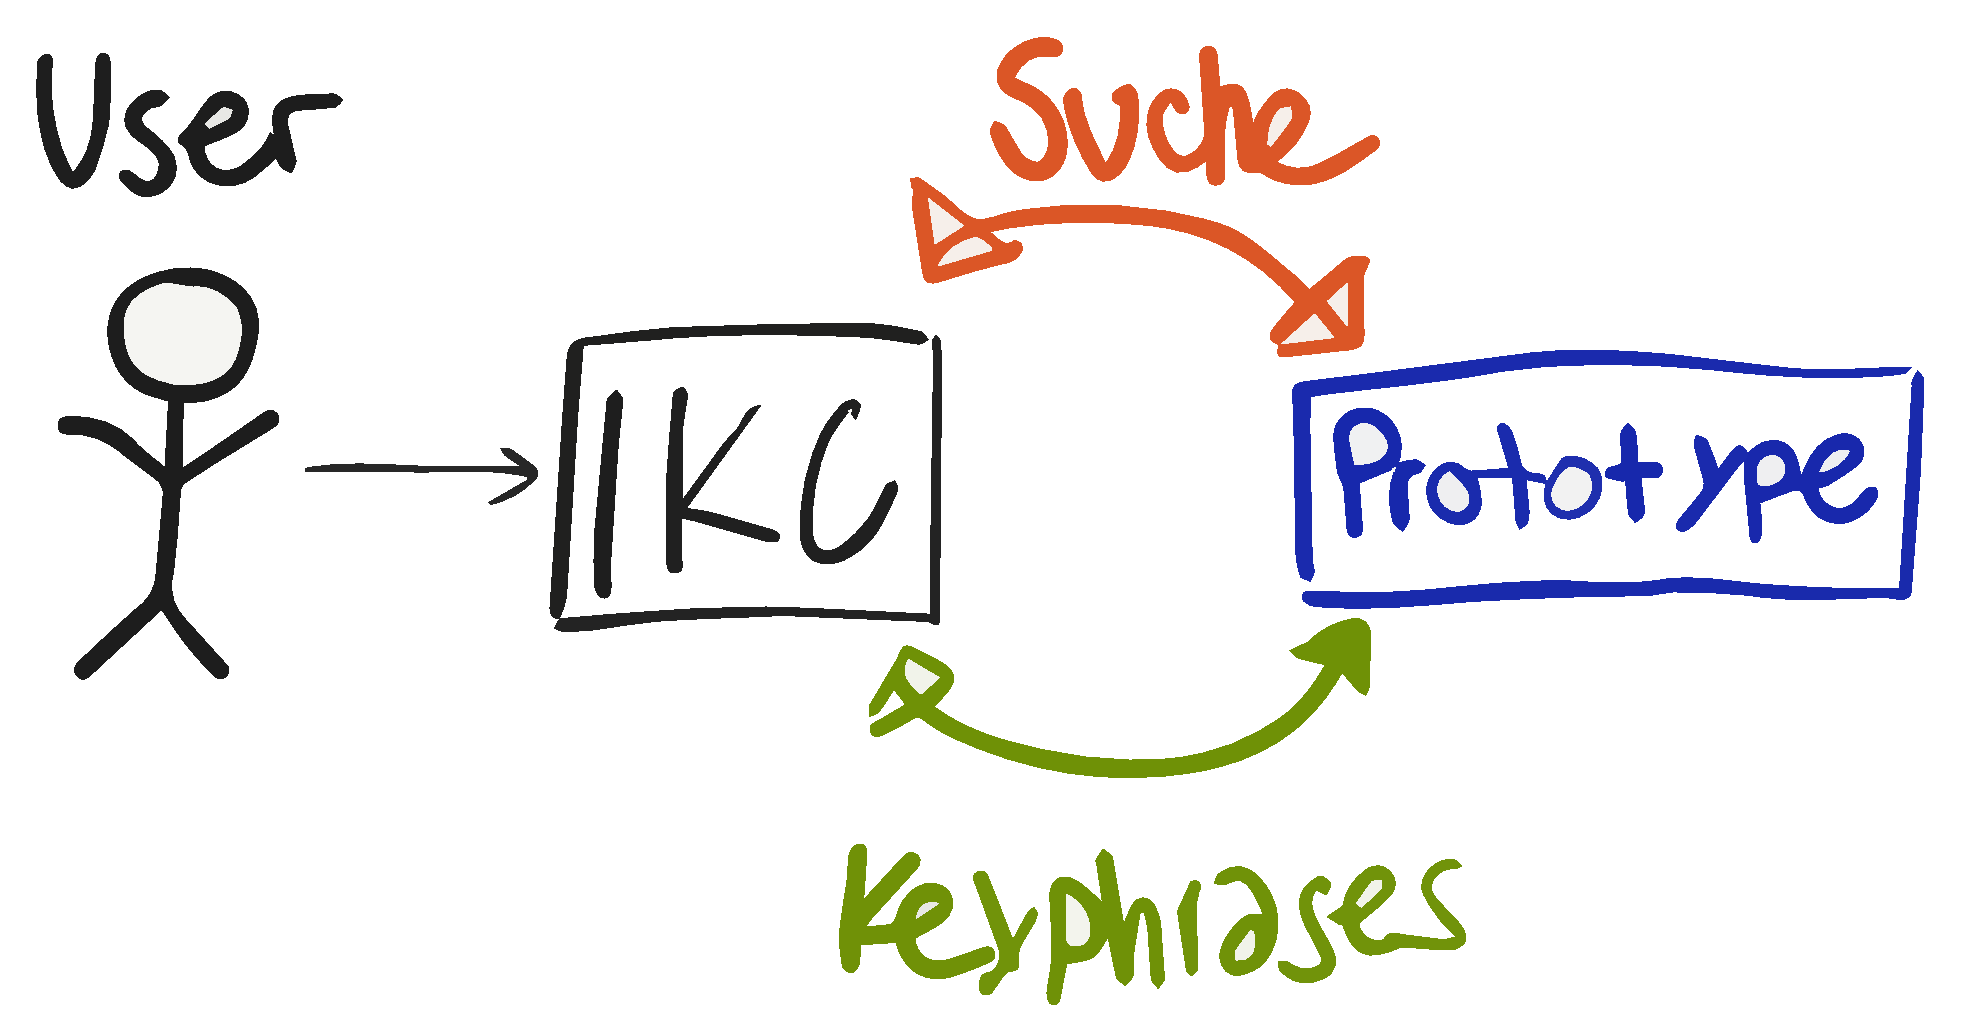
\includegraphics[width=0.6\textwidth]{kontext}
\caption{Kontextdiagramm}
\label{fig:kontextdiagramm}
\end{figure}

\gls{Keyphrase}[s] sind Begriffe, welche aus einem oder mehreren Wörtern bestehend und den zugrunde liegenden Text kurz und prägnant für den Benutzer zusammenfassen. Für weitere Informationen steht das Glossar zur Verfügung (\hyperref[glossar]{Kapitel Glossar}).

Basierend auf der Aufgabenstellung, dem Projekt-Kontext und den bestehenden Systemen definieren die folgenden Punkte die Ausgangslage:
\begin{itemize}
    \item Der bestehende Prototyp \gls{ikc-core} dient als Grundlage für diese Bachelorarbeit. Mit dem Fokus der reinen Datenanalyse wird auf die Datenquellen Dropbox und Evernote verzichtet. Der resultierende Prototyp baut auf der bestehenden Umgebung auf.
    \item Aufgrund der bisherigen Erfahrungen und dem bestehenden Code wird als Programmiersprache weiterhin \gls{Typescript} eingesetzt. Dies hat unter anderem den Vorteil, dass \gls{Typescript} sowohl client- als auch serverseitig lauffähig ist.
    \item Der Prototyp soll nach wie vor im Browser ausgeführt werden. Jegliche Daten werden nur an benutzerdefinierten Orten gespeichert. Es wird keine zusätzlich Persistenz eingeführt.
    \item Als Plattform wird weiterhin das Docker-basierte \gls{Dokku} eingesetzt. Dieses wird bereits für den Proof of Concept (\gls{PoC}) und für das Prototyping verwendet.
\end{itemize}

\section{Scope}\label{sec:scope} 
Zur Abgrenzung definiert der Scope den Inhalt und den Umfang eines Projektes. Für dieses Projekt ist er wie folgt festgelegt:
\begin{itemize}
    \item Da die Herkunft der Informationen für die Analyse nicht wichtig ist, beschränkt sich die Arbeit auf Text-Dateien. Versprechen die Resultate einen grossen Mehrwert, können die Konzepte spä\-ter für die Verwendung mit weiteren Datenquellen erweitert werden.
    \item Um mögliche Schwierigkeiten und Hindernisse mit Dropbox von Beginn an auszuschliessen, wird eine neue Datenquelle und Persistenzbasis auf der Grundlage von \gls{SFTP} eingeführt.
    \item Der Projektpartner stellt die Testdaten auf Basis einer Sammlung von Wikipedia-Artikeln zur Verfügung. Möglicherweise muss die Auswahl aufgrund der grossen Datenmenge ein\-ge\-schränkt werden.
    \item Aufgrund der Anforderungsanalyse\footnote{{Protokoll der Anforderungsanalyse \autoref{anforderungsanalyse-mk}}} mit dem Projektpartner wurde das Projekt noch spezifischer auf die Schlüss\-el\-wort\-ex\-traktion fokussiert. Ein \gls{SFTP}-Service ersetzt dabei eine Anbindung an Dropbox und Evernote komplett.
\end{itemize}

\section{Projektstrukturplan}
Die \autoref{fig:projektstrukturplan} gewährt einen Überblick über das Projekt. Sie stellt die wichtigsten Bereiche und Phasen dar, in welche die Arbeit grob eingegliedert werden kann:
\begin{enumerate}
    \item Die \textbf{Projektführung} beinhaltet die Planung des Vorhabens über den gegebenen Zeitraum. Ständige Kontrolle des Ist- gegenüber dem Soll-Zustand kann gegebenenfalls jederzeit zur Steuerung oder Anpassungen des Zeitplans führen. Da das Projekt agil organisiert ist, liegt das Augenmerk auf der Priorisierung der Anforderungen.
    \item In der \textbf{Konzeption} werden neben den Anforderungen auch vorstellbare Lös\-ungs\-an\-sätz\-e in den Bereichen Architektur sowie Schnittstellen geprüft.
    \item Nach einer anfänglichen Recherchephase werden zu Testzwecken bereits erste Prototypen entwickelt. So sollen mögliche Optionen überprüft und gegebenenfalls später implementiert oder weiterentwickelt werden. Nach einer \textbf{Evaluation} werden die geeigneten Lösungen ausgewählt.
    \item In der \textbf{Entwicklung} werden die gesammelten Erkenntnisse gesammelt und analysiert. Grundsätzlich soll auf den zuvor entwickelten Prototypen aufgebaut werden. Zunächst wird ei\-gen\-stän\-dig, ohne Einbindung in den \gls{ikc-core} entwickelt.
    \item Sobald die Implementierung die erforderlichen Anforderungen reibungslos erfüllt, wird sie in den bestehenden \gls{ikc-core} \textbf{integriert}. Nach letzten Optimierungen sind nun alle Anforderungen erfüllt und intensivere Tests können durchgeführt werden. Für die Entwicklung werden hauptsächlich Integrationstests verwendet.
    \item Nachdem die Entwicklungsarbeit abgeschlossen ist, folgt der \textbf{Projektabschluss}. Dabei wird die endgültige Version des Projektreports erstellt und die Abschlusspräsentation gehalten.
\end{enumerate}

\section{Rahmenplan}
Die Rahmenplanung, basierend auf dem Projektstrukturplan (\autoref{fig:rahmenplan}), repräsentiert die zeitliche Planung des Projekts. Dabei werden Kalenderwochen anstelle von Daten oder Schulwochen verwendet. Enthalten sind alle Projektphasen, Sprints und Meilensteine, als auch alle Lieferobjekte welche im \autoref{lieferobjekte} weiter ausgeführt werden. Die Dauer der Sprints wird bewusst unterschiedlich ausgestaltet, um den verschiedenen Projektphasen und deren Inhalten bestmöglich Rechnung zu tragen.
%Die Sprints dauern absichtlich unterschiedlich lange, das deshalb, weil die Länge auf\-grund der verschiedenen Projektphasen und deren Inhalt zugeordnet worden ist. Weiter werden administrative Elemente durch blaue Färbung und Entwicklungs-Elemente durch rote Färbung gekennzeichnet.

Ein wichtiger Teil der Rahmenplanung sind die Meilensteine. Sie unterteilen das Projekt in Phasen, welche dadurch klar voneinander getrennt sind. Ebenfalls sind sie eine wichtige Orientierungshilfe im Projekt und weisen den Weg zu einem erfolgreichen Abschluss. Sie werden in \autoref{tab:meilensteine} aufgelistet.

\section{Projektziele} \label{projektziele}
Projektziele werden definiert, um den Erfolg an ausgewählten Punkten zu überprüfen und sicherstellen. Sie wurden in Absprache mit dem Projektpartner definiert. Die Ziele sind in der folgenden \autoref{tab:projekt-ziele} aufgelistet und anschliessend genauer ausgeführt.


%1.) Den Volltext von Dropbox-Dateien und Evernote-Notizen in IKC zu durchsuchen
%2.) Relevante Schlüsselwörter pro Dokument zu ext-rahieren
%3.) Schlüsselwörter automatisch dem Wissensnetz-werk hinzuzufügen
%4.) Dokumente mit den Schlüsselwörtern automatisch zu verknüpfen.

\begin{longtable}{|p{1cm}  | p{10.5cm}|}
  \hline
    ID & Beschreibung \\\hline
    Z1 & Volltextsuche zusätzlich über externe Inhalte.\\\hline
    Z2 & Pro Dokument relevante \gls{Keyphrase}[s] extrahieren.\\\hline
    Z3 & Extrahierte \gls{Keyphrase}[s] werden automatisch dem Wissensnetzwerk hinzugefügt.\\\hline
    Z4 & Dokumente werden automatisch mit den entsprechenden \gls{Keyphrase}[s] verbunden.\\\hline
    \caption{Projektziele}
  \label{tab:projekt-ziele}
\end{longtable}

\begin{enumerate}
    \item \textbf{Z1}: Der Prototyp bietet eine Volltextsuche über den gesamten Inhalt der Dokumente einer externen Datenquelle an. Die Suchfunktion ist in den \gls{ikc-core} integriert.
    \item \textbf{Z2}: Zu den einzelnen Dokumenten extrahiert der Prototyp aus dem Text relevante \gls{Keyphrase}[s].
    \item \textbf{Z3}: Diese \gls{Keyphrase}[s] werden nach der Extraktion direkt Teil des Wissensnetzwerkes. Diese können vom Benutzer wieder entfernt werden.
    \item \textbf{Z4}: Sowohl \gls{Keyphrase} als auch Dokument werden als Node innerhalb des \gls{ikc-core} repräsentiert und sind miteinander verbunden. 
\end{enumerate}

\section{Anforderungen} \label{sec:anforderungen}

Für die weitere Unterteilung in Arbeitspakete und \textit{Stories} werden die Anforderungen zunächst in Prosa gesammelt. Diese entstammen dem Kundenworkshop und der Aufgabenstellung. Sie widerspiegeln die Projektziele (\autoref{projektziele}). Die Anforderungen werden in funktionale und nicht-funktionale Anforderungen unterschieden. Die funktionalen Anforderungen definieren direkt die Eigenschaften. Im Gegensatz dazu definieren nicht-funktionale Anforderungen die Leistung und die Randbedingungen. Diese sind in der Tabelle \autoref{tab:funktionale-anforderungen}, beziehungsweise \autoref{tab:nicht-funktionale-anforderungen} zu finden.

Die Priorisierung erfolgt nach dem \gls{MoSCoW-System}:

\begin{longtable}{|p{1.5cm} | p{2.5cm} | p{7.2cm}|}
  \hline
    \# & Priorität & Beschreibung \\\hline
    M & Must Have & Bei dieser Anforderung handelt es sich um ein Muss, höchste Priorität.\\\hline
    S & Should Have & Diese Anforderung wird erwartet, normale Priorität.\\\hline
    C & Could Have & Tiefste Priorität, desiderata.\\\hline
    \caption{MosCow-Priorisierung}
  \label{tab:moscow}
\end{longtable}


Neben den in der Aufgabenstellung vorgegebenen Lieferobjekte (\autoref{tab:set-lieferobjekte}) sind noch zusätzliche, interne Lieferobjekte (\autoref{tab:add-lieferobjekte}) festlegt. Diese sind lediglich als Unterstützung der Projektkontrolle, eine Art Orientierungshilfe, gedacht.
